\section{Methods}

The ability of liquid-fueled systems to continuously remove fission products and add 
fissile and/or fertile elements is the main challenge for depletion simulations. 
The python package introduced in this work, SaltProc, takes into account online 
separations and feeds using the SERPENT 2 continuous-energy Monte Carlo neutron 
transport and depletion code. In this work, all figures of the core model
were generated using the built-in SERPENT 2 plotter. 

\subsection{Molten Salt Breeder Reactor design and model description}
The \gls{MSBR} vessel has a diameter of 680 cm and a height of 610 cm. It 
contains a molten fluoride fuel-salt mixture that generates heat in the active 
core region and transports that heat to the primary heat exchanger by way of 
the primary salt pump. In the active core region, the fuel salt flows through 
channels in moderating and reflecting graphite blocks. Fuel salt at
565$^{\circ}$C enters the central manifold at the bottom via four 
40.64-cm-diameter nozzles and flows upward through channels in the lower plenum 
graphite. The fuel salt exits at the top at about 704$^{\circ}$C through four 
equally spaced nozzles which connect to the salt-suction pipes leading to 
primary circulation pumps. The fuel salt drain lines connect to the bottom of 
the reactor vessel inlet manifold.

Figure~\ref{fig:serpent_plan_view} shows the configuration of the 
\gls{MSBR} vessel, including the ``fission" (zone I) and ``breeding" 
(zone II) regions inside the vessel. The core has two radial zones bounded by a 
solid cylindrical graphite reflector and the vessel wall. The central zone, 
zone I, in which 13\% of the volume is fuel salt and 87\% graphite, is
composed of 1,320 graphite cells, 2 graphite control rods, and 2 
safety\footnote{ These rods needed for emergency shutdown only.} rods. The 
under-moderated zone, zone II, with 37\% fuel salt, and radial reflector, 
surrounds the zone I core region and serves to diminish neutron leakage. Zones 
I and II are surrounded radially and axially by fuel salt 
(figure~\ref{fig:serpent_zoneII}). This space for fuel is necessary for 
injection and flow of molten salt.

\begin{figure}[hbp!] % replace 't' with 'b' to \centering
  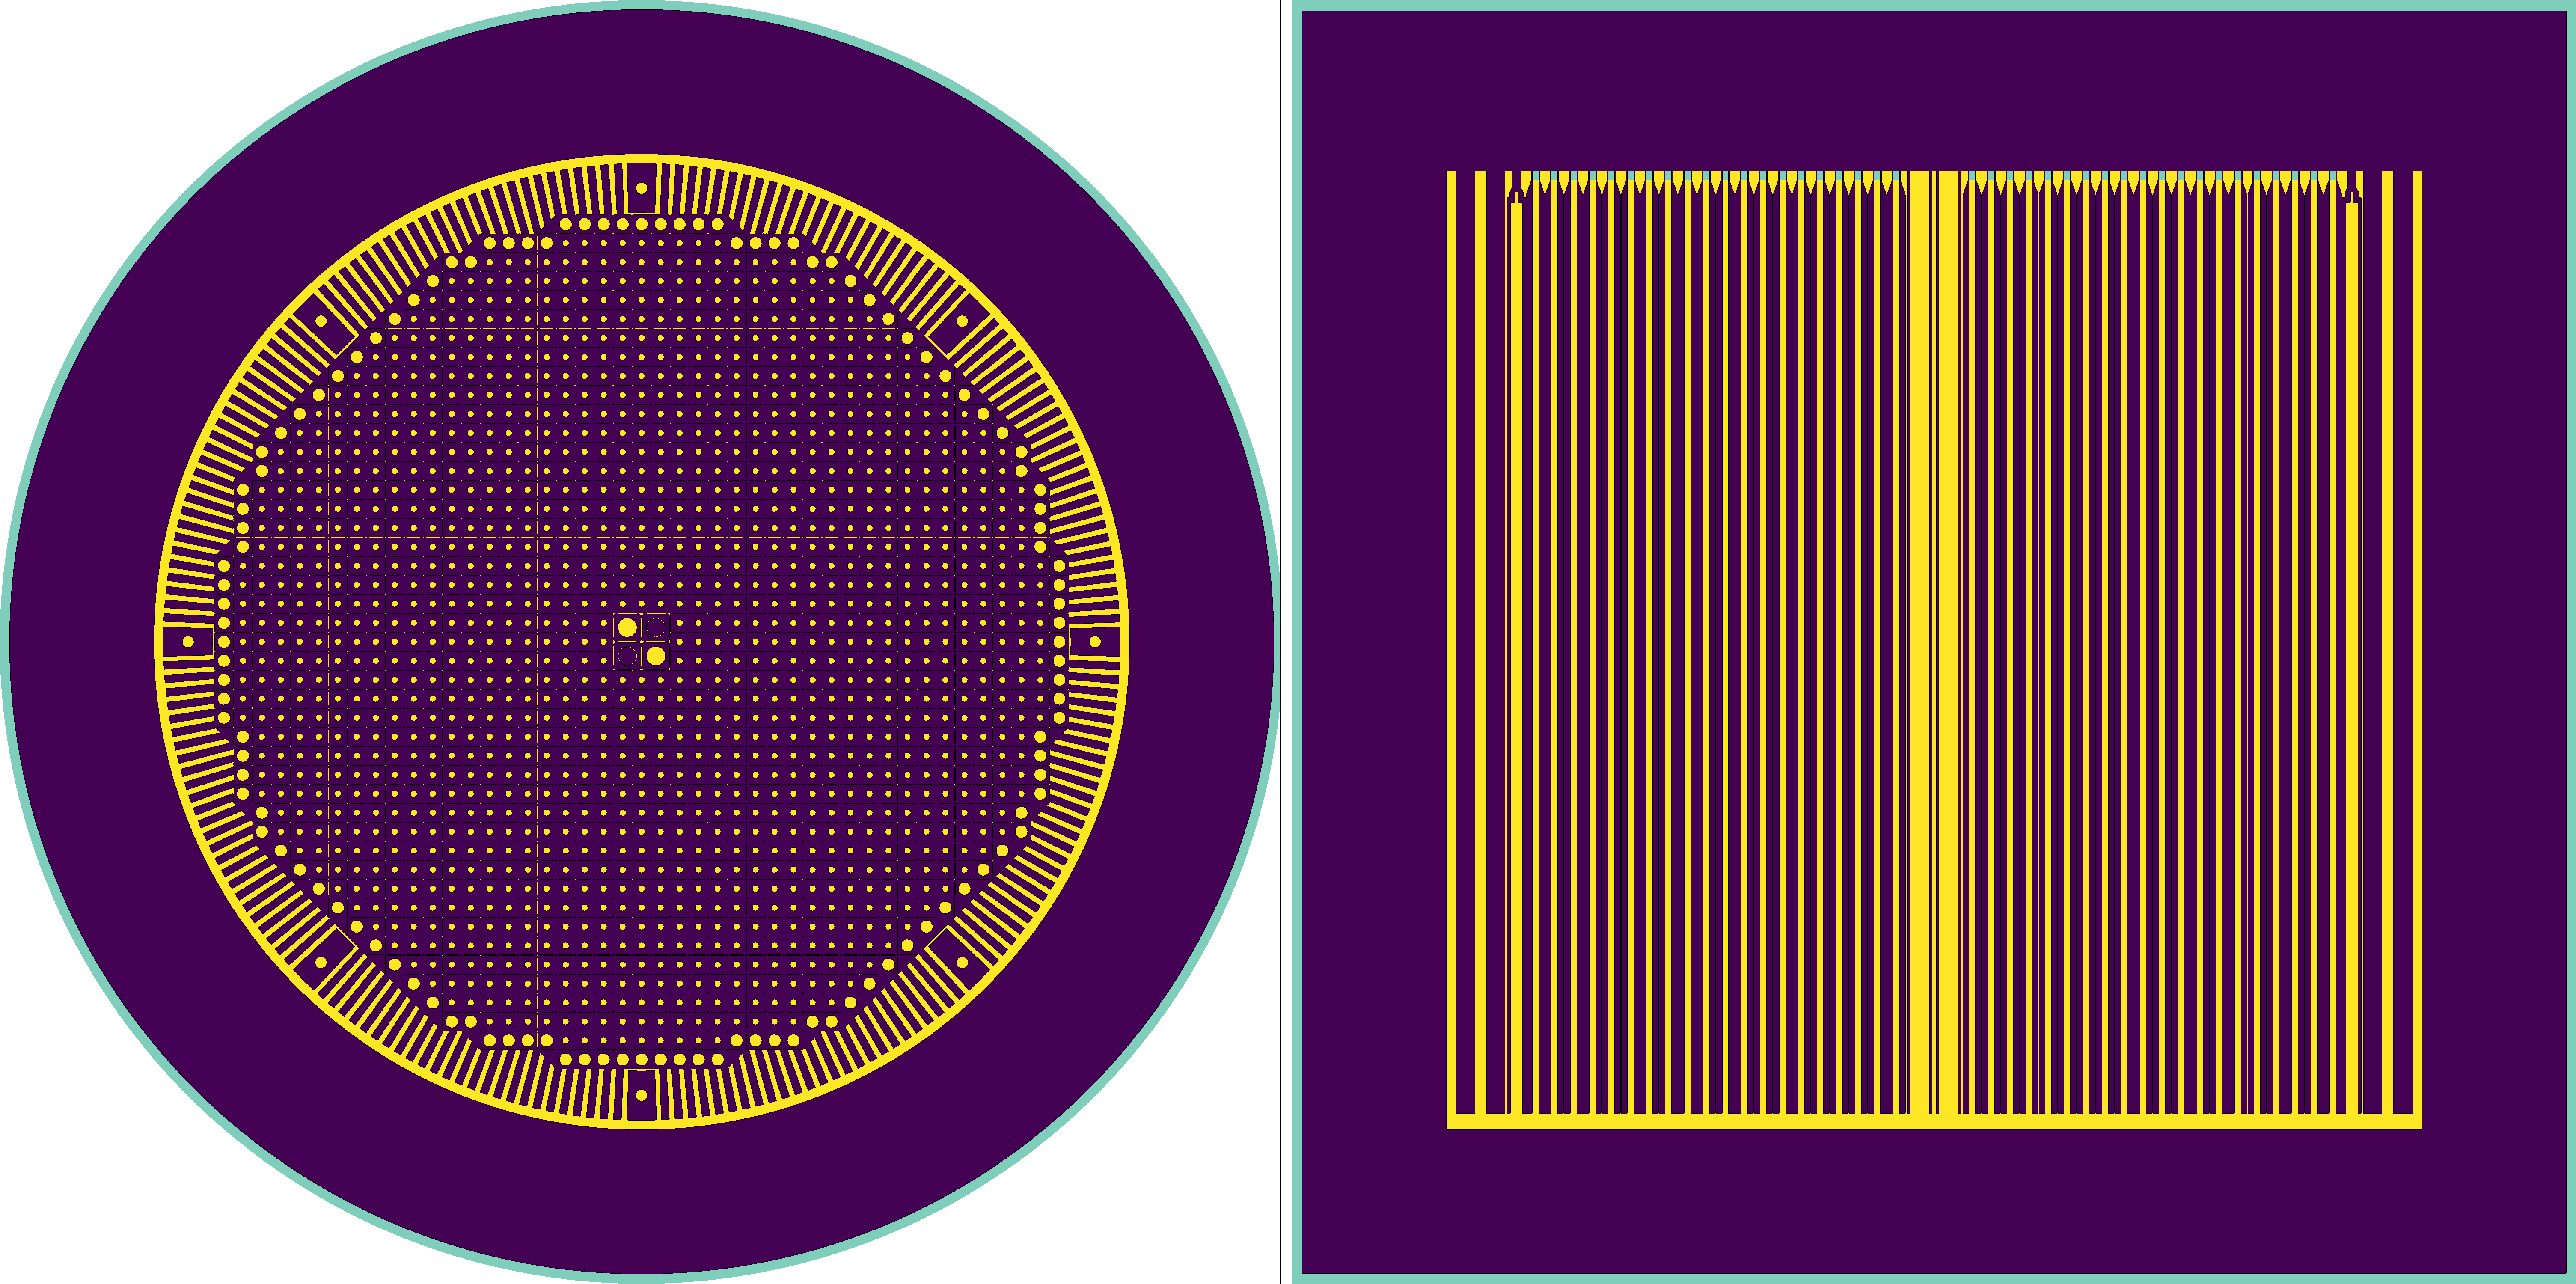
\includegraphics[width=\textwidth]{view_serpent.png}
  \caption{Plan and elevation views of SERPENT 2 \gls{MSBR} model developed in 
  this work.}
  \label{fig:serpent_plan_view}
\end{figure}

\begin{figure}[t!] % replace 't' with 'b' to \centering
  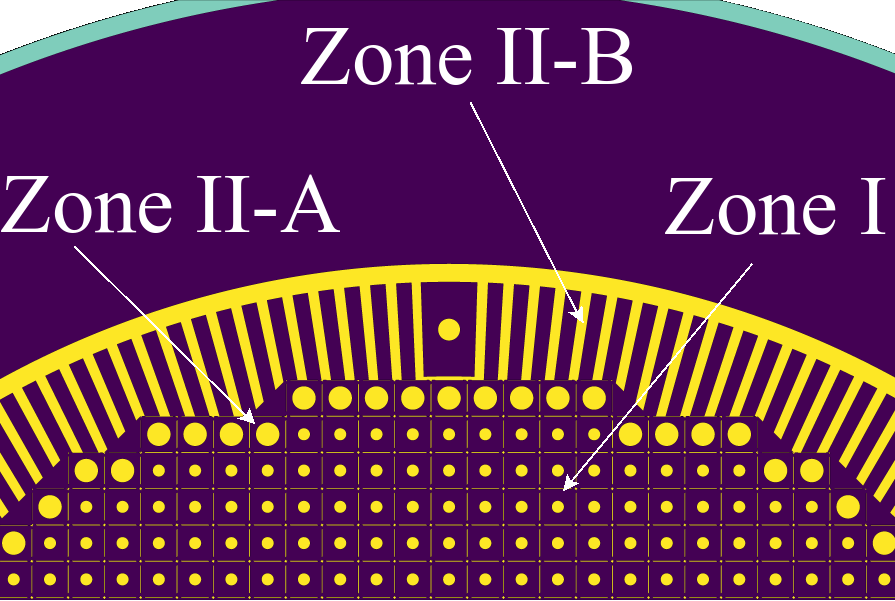
\includegraphics[width=\textwidth]{ser_zone_II.png}
  \caption{Detailed view of \gls{MSBR} two zone model. 
          Yellow represents fuel salt, purple represents graphite, and aqua represents the reactor vessel.}
  \label{fig:serpent_zoneII}
\end{figure}

Since reactor graphite experiences significant dimensional changes due to 
neutron irradiation, the reactor core was designed for periodic replacement. 
Based on the experimental irradiation data from the \gls{MSRE}, the core graphite 
lifetime is about 4 years and the reflector graphite lifetime is 30 years 
\cite{robertson_conceptual_1971}.

There are eight symmetric graphite slabs with a width of 15.24 cm in zone II, 
one of which is illustrated in Figure~\ref{fig:serpent_zoneII}. The holes in 
the centers are for the core lifting rods used during the core replacement 
operations. These holes also allow a portion of the fuel salt to flow to the 
top of the vessel for cooling the top head and axial reflector. 
Figure~\ref{fig:serpent_zoneII} also shows
the 5.08-cm-wide annular 
space between the removable core graphite in zone II-B and the permanently 
mounted reflector graphite. This annulus consists entirely of fuel salt, 
provides space for moving the core assembly, helps compensate for the elliptical 
dimensions of the reactor vessel, and serves to reduce the damaging flux at the 
surface of the graphite reflector blocks. 

\subsubsection{Core zone I}
The central region of the core, called zone I, is made up of graphite elements, 
each $10.16$cm$\times$10.16cm$\times$396.24cm. Zone I has 4 channels for 
control rods: two for graphite rods which both regulate and shim during normal 
operation, and two for backup safety rods consisting of boron carbide clad to 
assure sufficient negative reactivity for emergency situations.

These graphite elements have a mostly rectangular shape with lengthwise ridges 
at each corner that leave space for salt flow elements. Various element sizes 
reduce the peak damage flux and power density in the center of the core to 
prevent local graphite damage.  Figure~\ref{fig:I_element_ref} shows the 
elevation and plan views of graphite elements of zone I 
\cite{robertson_conceptual_1971} and their SERPENT model 
\cite{rykhlevskii_full-core_2017}.

\begin{figure}[ht!] % replace 't' with 'b' to \centering
  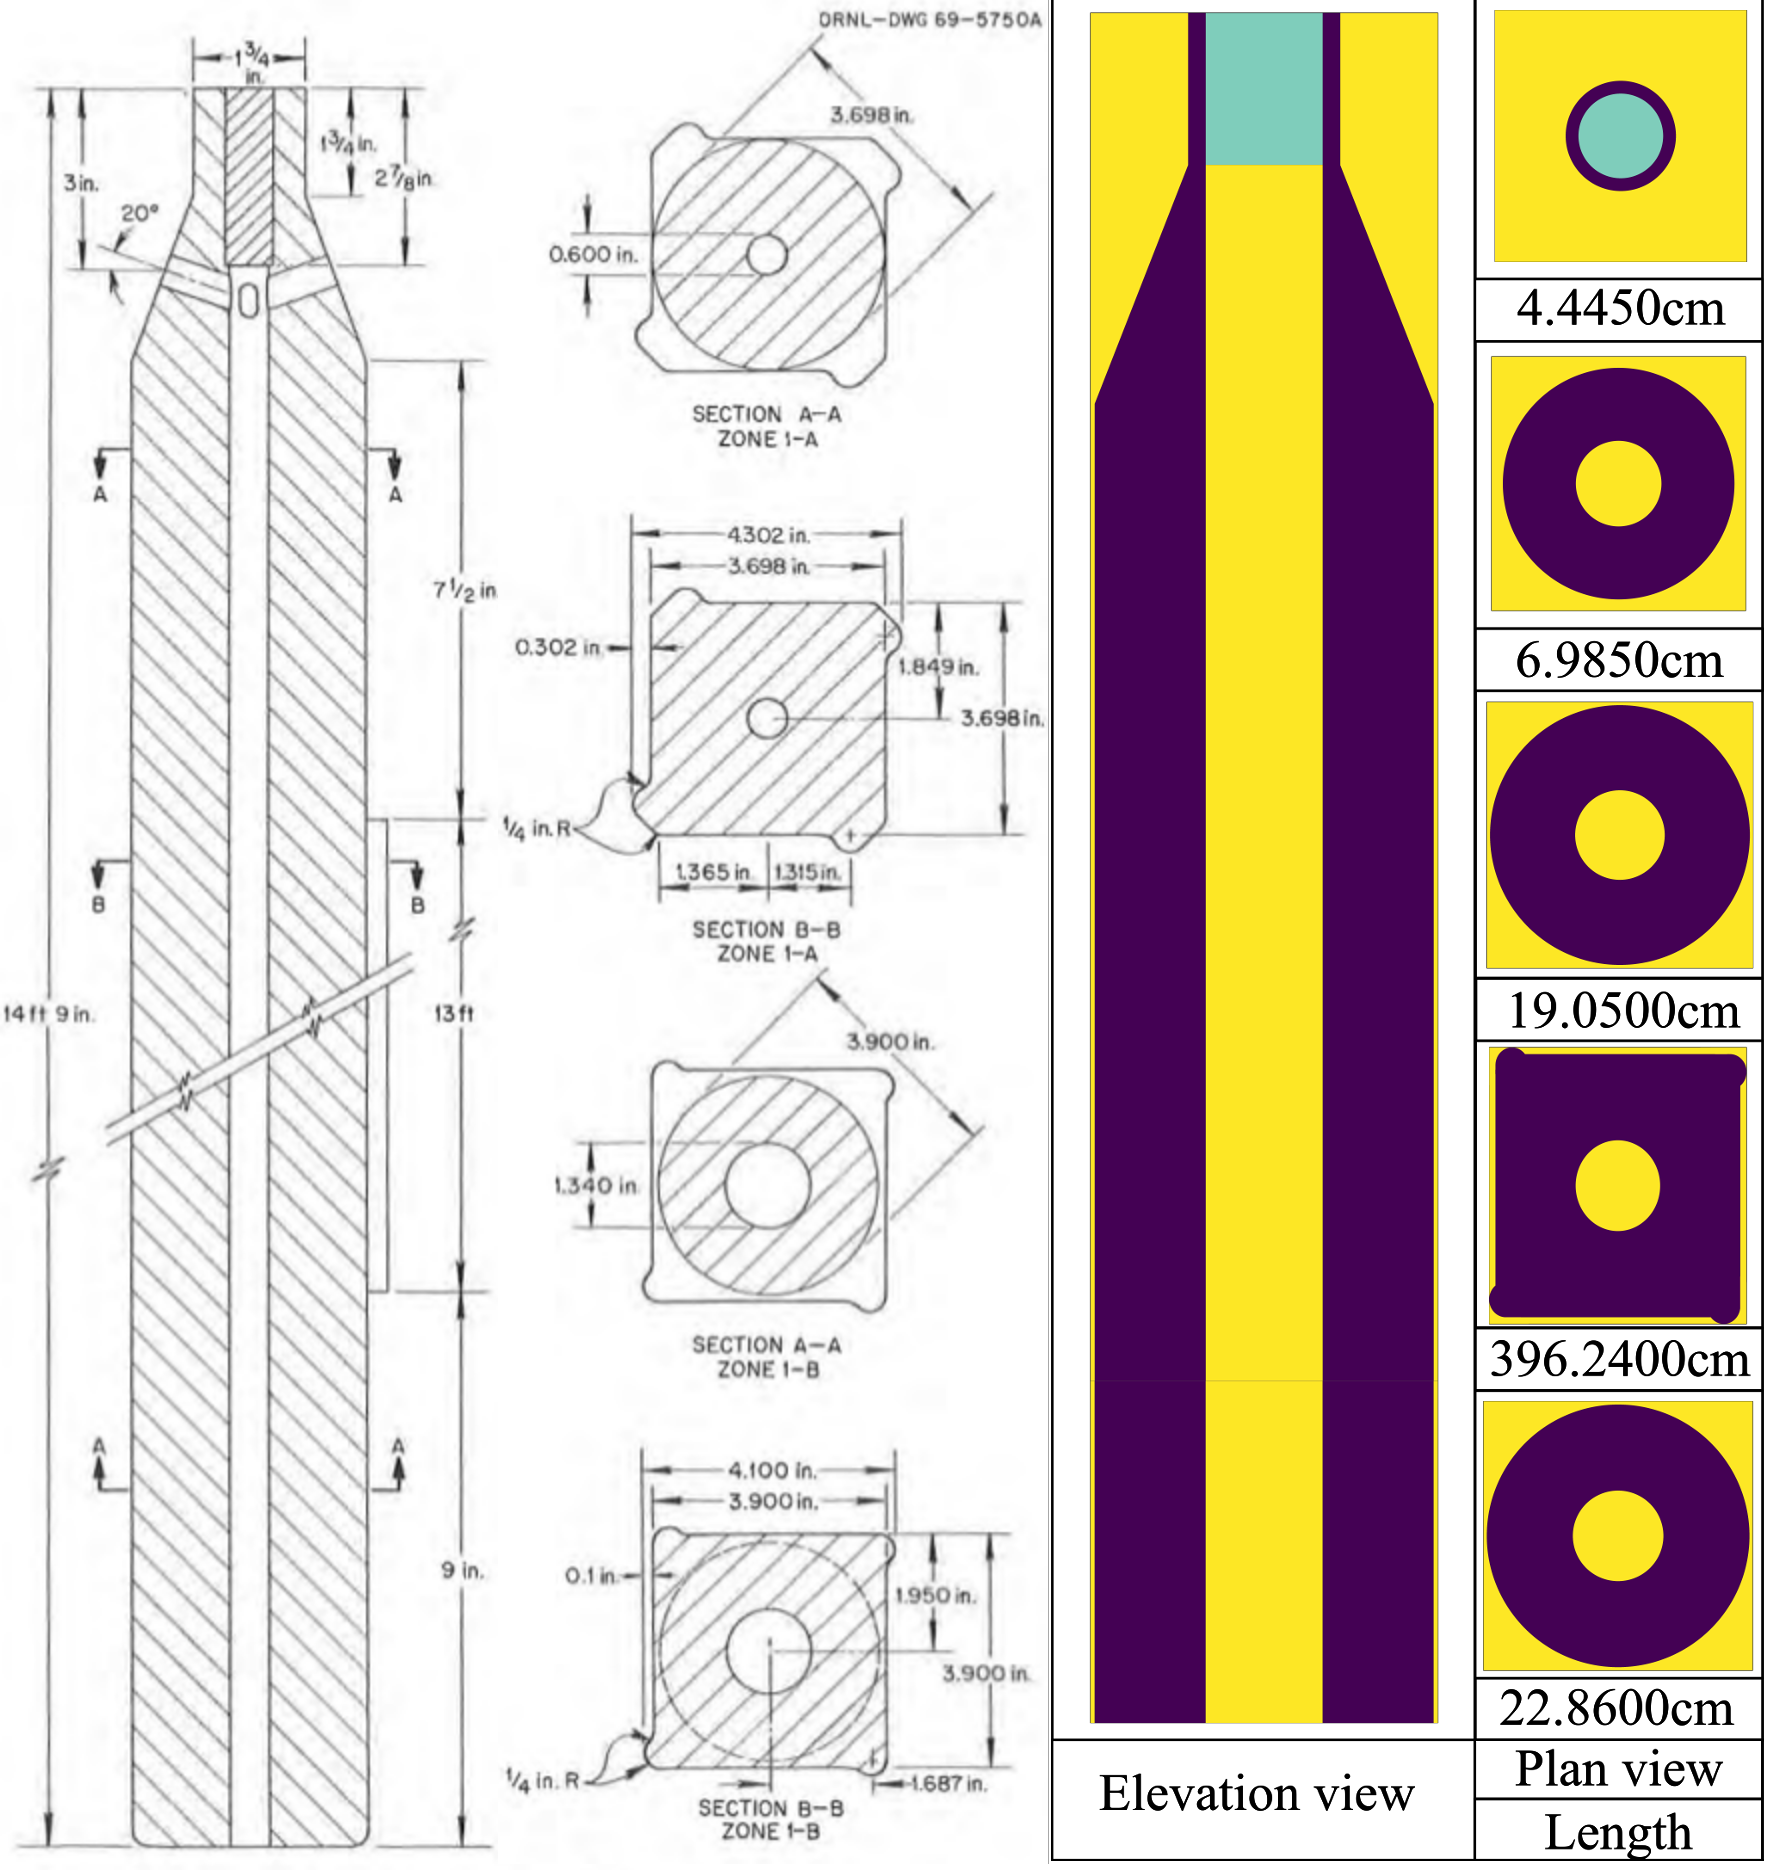
\includegraphics[width=\textwidth]{zone_I_element_ref.png}
  \caption{Graphite moderator elements for zone I 
  \cite{robertson_conceptual_1971,rykhlevskii_full-core_2017}.  Yellow 
  represents fuel salt, purple represents graphite, and aqua represents the 
  reactor vessel.}
  \label{fig:I_element_ref}
\end{figure}

\subsubsection{Core zone II}
Zone II, which is undermoderated, surrounds zone I. Combined with the bounding 
radial reflector, zone II serves to diminish neutron leakage. Two kinds of 
elements form this zone: large-diameter fuel channels (zone II-A) and 
radial graphite slats (zone II-B). 

Zone II has 37\% fuel salt by volume and each element has a fuel channel 
diameter of 6.604cm. The graphite elements for zone II-A are prismatic with
elliptical dowels running axially between the prisms. These dowels
isolate the fuel salt flow in zone I from that in zone II. 
Figure~\ref{fig:II_element_ref} shows the shapes and dimensions of these graphite 
elements and their SERPENT model. Zone II-B elements are rectangular slats 
spaced far enough apart to provide the 0.37 fuel salt volume fraction. The 
reactor zone II-B graphite 5.08cm-thick slats vary in the radial dimension 
(average width is 26.67cm) as shown in figure~\ref{fig:serpent_zoneII}. Zone II 
serves as a blanket to achieve the best performance: a high breeding ratio and 
a low fissile inventory. The harder neutron energy spectrum in zone II 
enhances the rate of thorium resonance capture relative to the fission rate, 
thus limiting the neutron flux in the outer core zone and reducing the neutron 
leakage \cite{robertson_conceptual_1971}. 

The sophisticated, irregular shapes of the fuel elements challenge an accurate 
representation of zone II-B.  
The suggested design \cite{robertson_conceptual_1971} of zone II-B has 8 
irregularly-shaped graphite elements as well as dozens of salt channels. 
These graphite elements were simplified into right-circular cylindrical shapes  
with central channels. Figure~\ref{fig:serpent_zoneII} illustrates this core 
region in the SERPENT model. The volume of fuel salt in zone II was kept 
exactly at 37\%, so that this simplification did not considerably change the core 
neutronics. Simplyfying the eight edge channels was the only simplification made 
to the \gls{MSBR} geometry in this work. 

\begin{figure}[ht!] % replace 't' with 'b' to \centering
  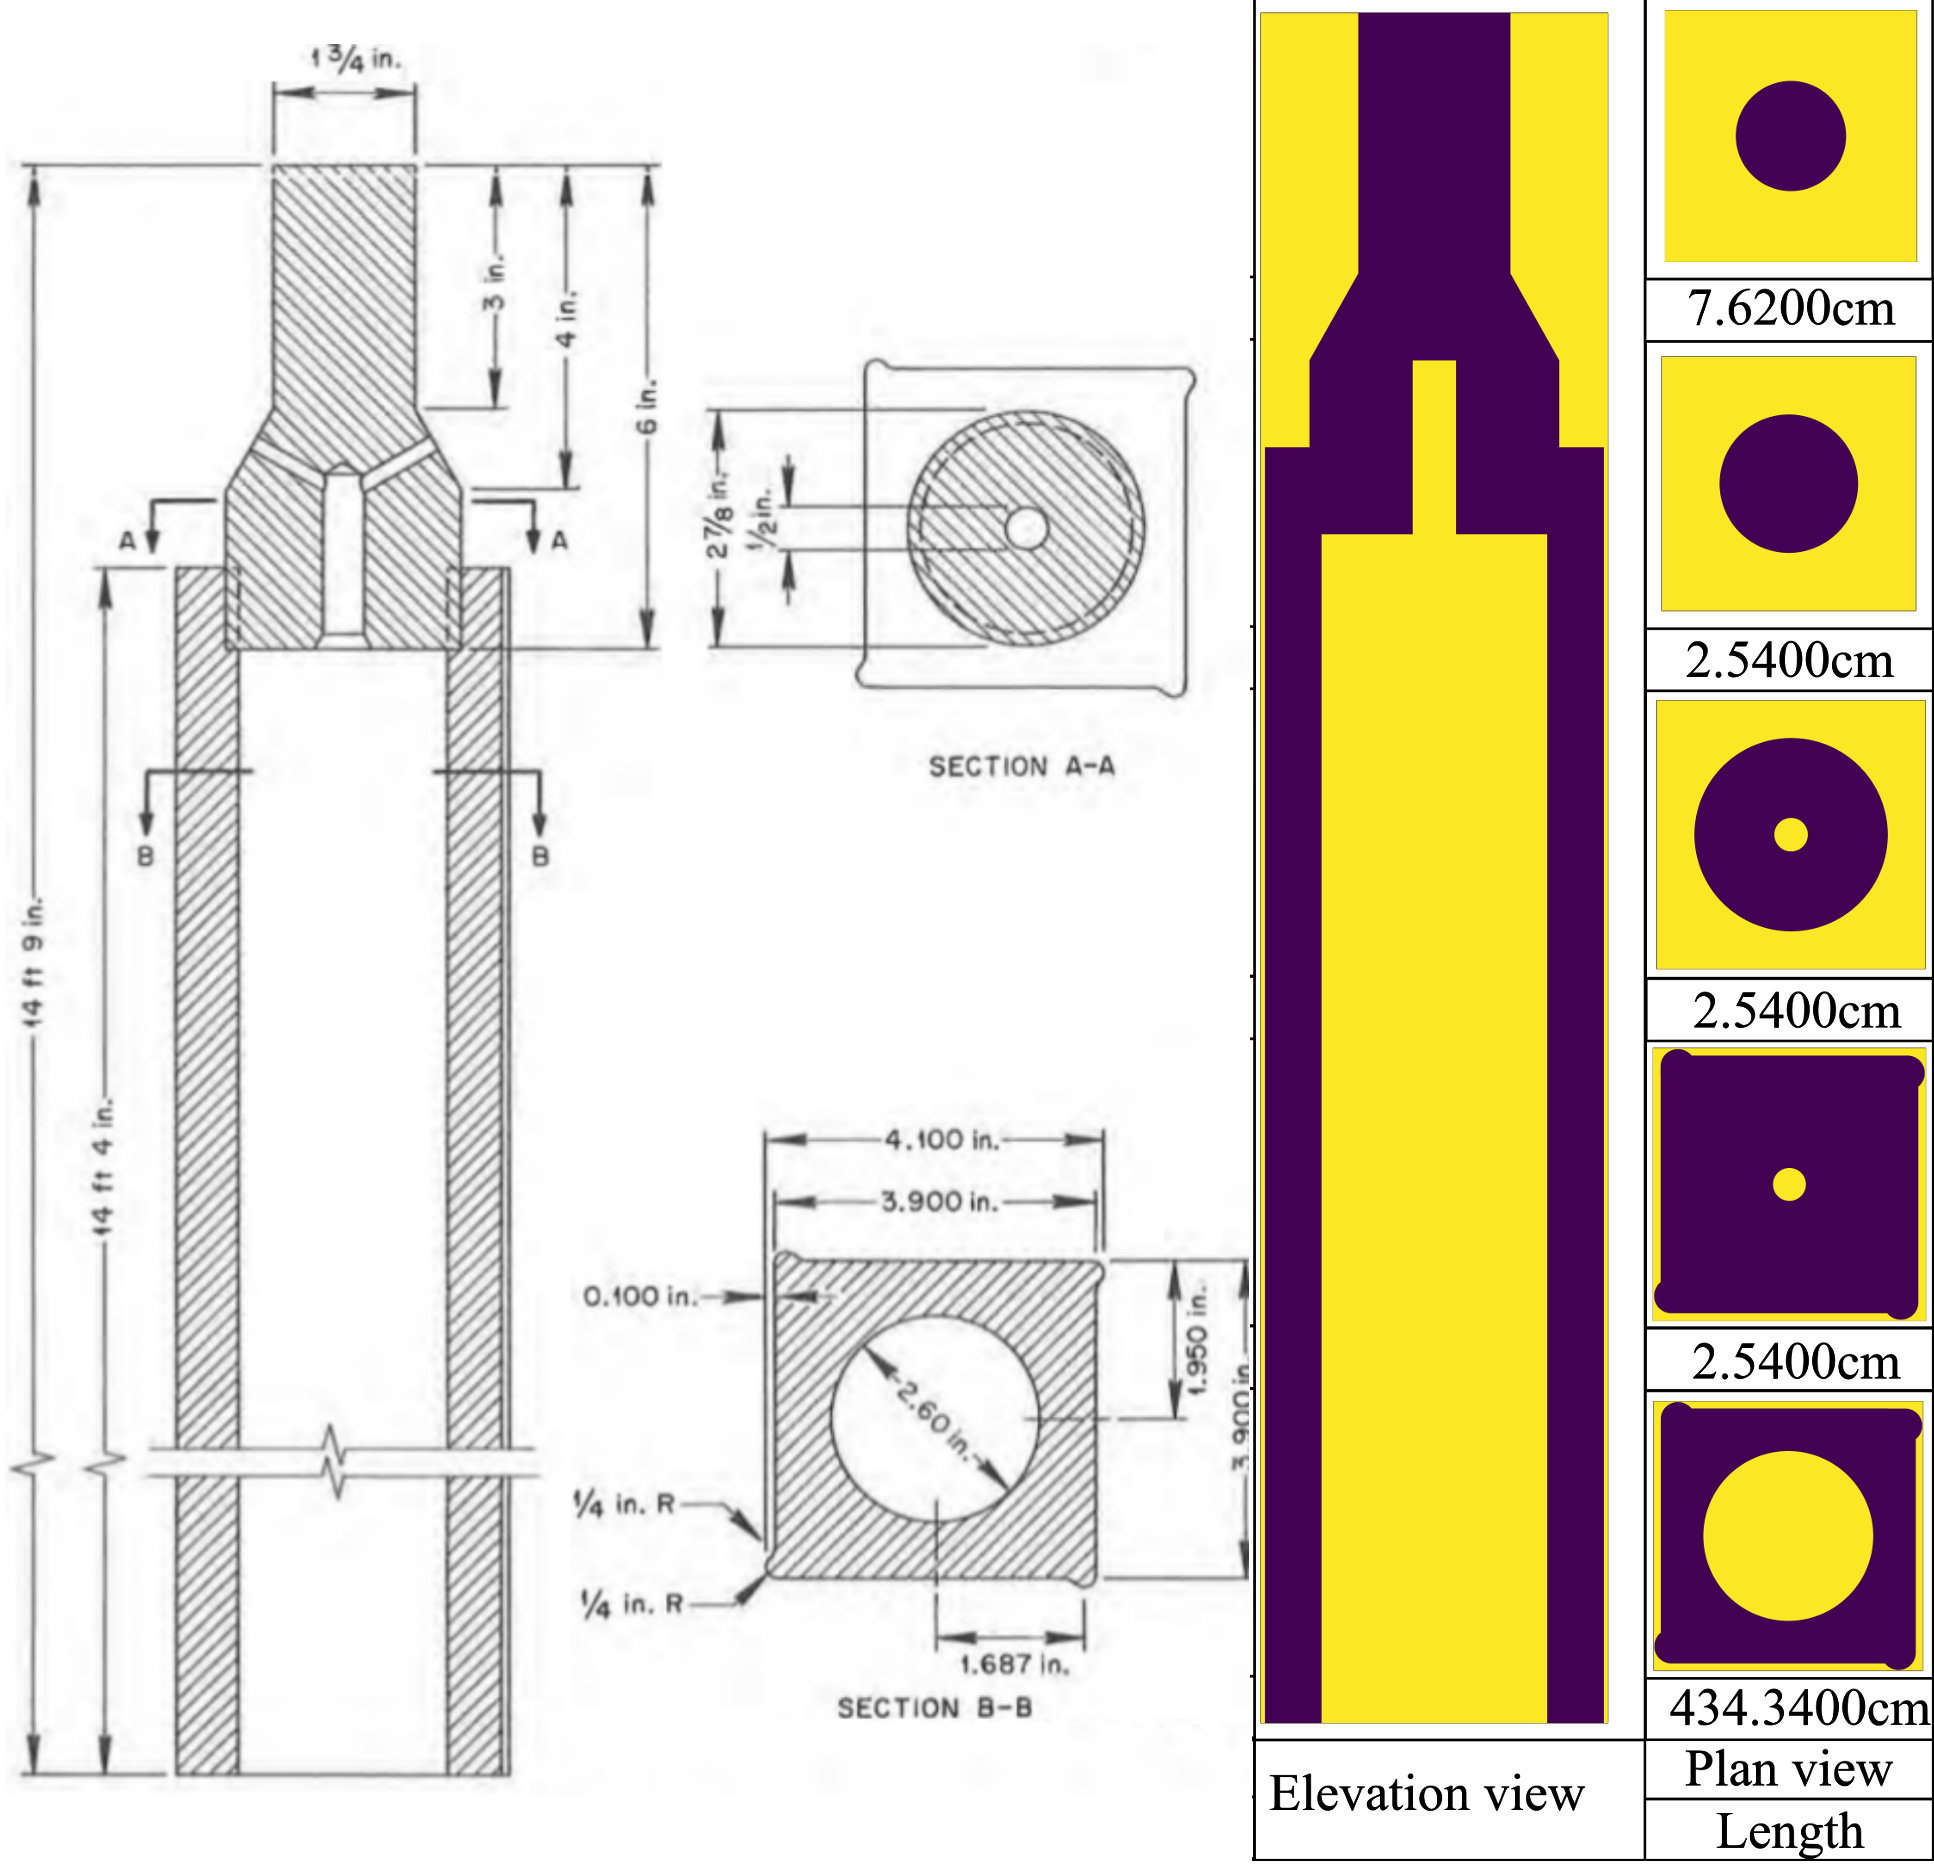
\includegraphics[width=\textwidth]{zone_II_element_ref.png}
  \caption{Graphite moderator elements for zone II-A 
  \cite{robertson_conceptual_1971,rykhlevskii_full-core_2017}.  Yellow 
  represents fuel salt and purple represents graphite.}
  \label{fig:II_element_ref}
\end{figure}

\subsubsection{Material composition and normalization parameters}
The fuel salt, reactor graphite, and modified Hastelloy-N
are all materials created at \gls{ORNL} specifically for the \gls{MSBR}.
The initial fuel salt used the same 
density (3.35 g/cm$^3$) and composition LiF-BeF$_2$-ThF$_4$-$^{233}$UF$_4$ 
(71.75-16-12-0.25 mole \%) as the \gls{MSBR} design 
\cite{robertson_conceptual_1971}. The lithium in the molten salt fuel is fully 
enriched to 100\% $^{7}$Li because $^{6}$Li is a very strong neutron poison and 
becomes tritium upon neutron capture. 

The JEFF-3.1.2 neutron library provided cross section generation 
\cite{oecd/nea_data_bank_jeff-3.1.2_2014}. 
The specific temperature was fixed 
for each material to correctly model the Doppler-broadening of resonance peaks 
when SERPENT generates the problem-dependent nuclear data library. The isotopic 
composition of each material at the initial state was described in detail in 
the MSBR conceptual design study \cite{robertson_conceptual_1971} and has been 
applied to the SERPENT model without any modification. Table~\ref{tab:msbr_tab} is 
a summary of the major \gls{MSBR} parameters used by this model 
\cite{robertson_conceptual_1971}. 

%%%%%%%%%%%%%%%%%%%%%%%%%%%%%%%%%%%%%%%%
\begin{table}[h!]
        %\centering
        \caption{Summary of principal data for \gls{MSBR} 
        \cite{robertson_conceptual_1971}.}
        \begin{tabularx}{\textwidth}{ s  s}
        \hline
                Thermal capacity of reactor           		& 2250 MW(t)
                \\ Net electrical output                 		& 1000 
        MW(e) \\  Net thermal efficiency        				
        & 44.4\%
                \\  Salt volume fraction in central zone I		& 0.13
                \\ Salt volume fraction in outer zone II       & 0.37
                \\ Fuel salt inventory (Zone I)                & 8.2 m$^3$	
        \\ Fuel salt inventory (Zone II)               & 10.8 m$^3$	\\ Fuel 
        salt inventory (annulus)               & 3.8 m$^3$	\\  Total fuel 
        salt inventory                   & 48.7 m$^3$	\\ Fissile mass in fuel 
        salt                   & 1303.7 kg	\\ Fuel salt components                  
                               & LiF-BeF$_2$-ThF$_4$-$^{233}$UF$_4$	\\  
        Fuel salt composition                 & 71.75-16-12-0.25 mole\%
                \\
                Fuel salt density                    & 3.35 g/cm$^3$
                \\ \hline
        \end{tabularx}
        \label{tab:msbr_tab}
\end{table}
%%%%%%%%%%%%%%%%%%%%%%%%%%%%%%%%%%%%%%%%%%%%%%%%

\subsection{Online reprocessing method}
Removing specific chemical elements from a molten salt 
requires intelligent design (e.g., chemical separations equipment design, 
fuel salt flows to equipment) and has a considerable economic cost. All 
liquid-fueled \gls{MSR} designs involve varying levels of online fuel 
processing. Minimally, volatile gaseous fission products (e.g. Kr, Xe) escape 
from the fuel salt during routine reactor operation and must be captured. 
Additional systems might be used to enhance removal of those elements. Most 
designs also call for the removal of noble and rare earth metals from the core 
since these metals act as neutron poisons. Some designs suggest a more complex 
list of elements to process (figure~\ref{fig:periodic_tab}), including the 
temporary removal of protactinium or other regulation of the 
actinide inventory \cite{ahmad_neutronics_2015}.

\begin{figure}[htp!] % replace 't' with 'b' to \centering
  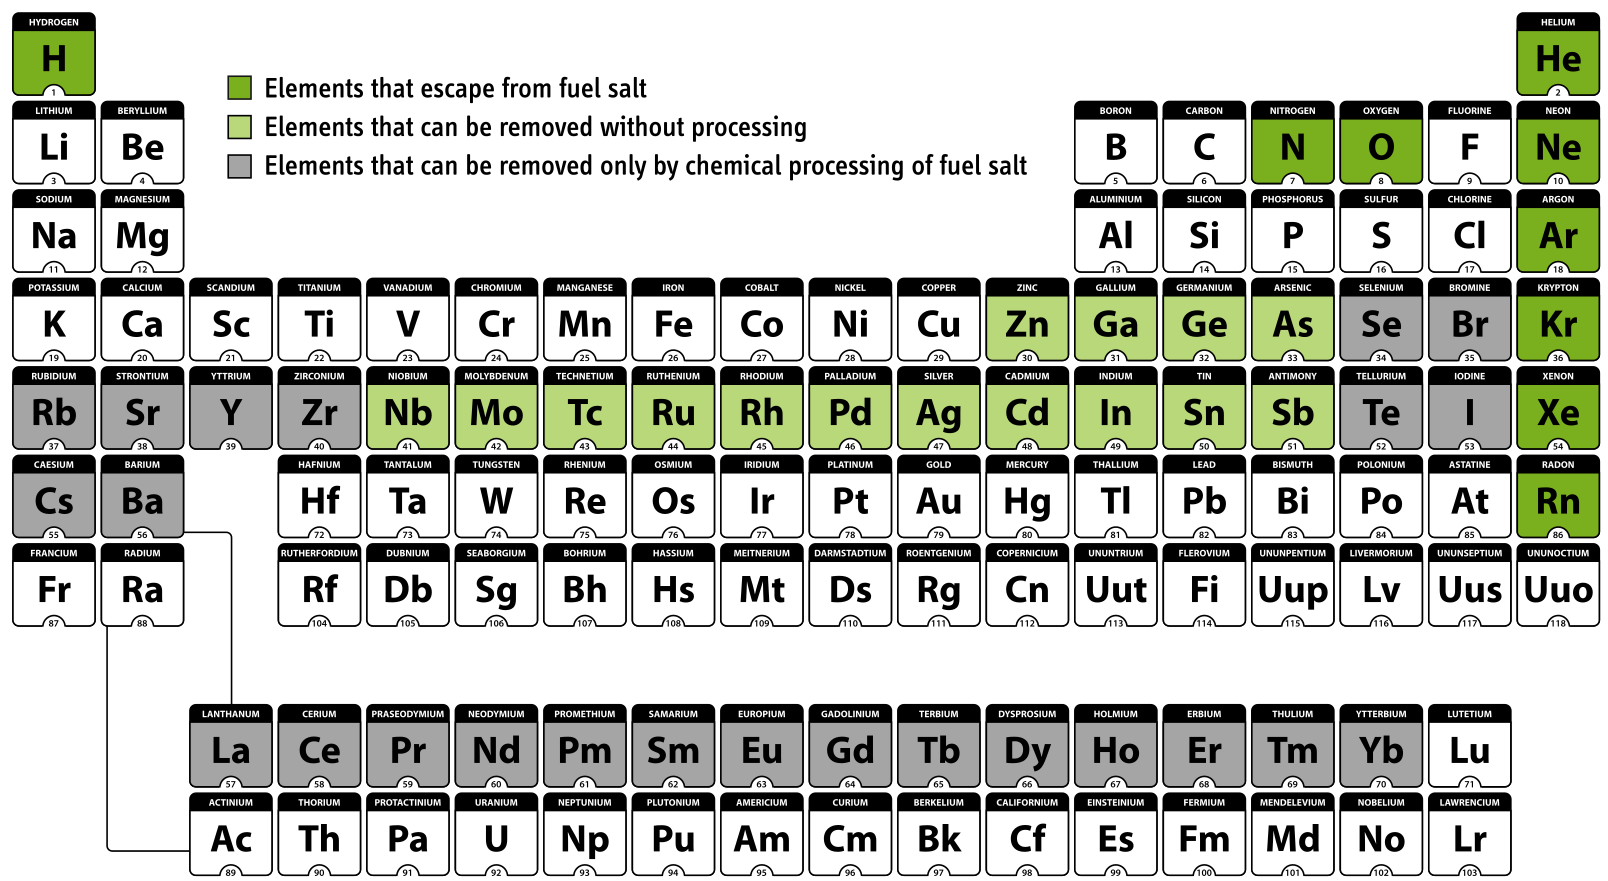
\includegraphics[width=\textwidth]{periodic_map.png}
  \caption{Processing options for \gls{MSR} fuels. 
          Reproduced from \cite{ahmad_neutronics_2015} where it was adapted 
          from a chart courtesy of Nicolas 
          Raymond, www.freestock.ca.}
  \label{fig:periodic_tab}
\end{figure}

\subsubsection{Fuel material flows}
The $^{232}$Th in the fuel absorbs thermal neutrons and produces $^{233}$Pa 
which then decays into the fissile $^{233}$U. Furthermore, the \gls{MSBR} 
design requires online reprocessing to remove all poisons (e.g. $^{135}$Xe), 
noble metals, and gases (e.g. $^{75}$Se, $^{85}$Kr) every 20 seconds. 
Protactinium presents a challenge, since it has a large absorption cross 
section in the thermal energy spectrum. Moreover, $^{233}$Pa left in the core
 would produce $^{234}$Pa and $^{234}$U, which both are not useful as fuel, 
and smaller amount of $^{233}$Pa would decays into the fissile $^{233}$U.
Accordingly, $^{233}$Pa is continuously 
removed from the fuel salt into a protactinium decay tank to allow $^{233}$Pa 
to decay to $^{233}$U without negative impact on neutronics. The reactor 
reprocessing system must separate $^{233}$Pa from the molten-salt fuel over 3 
days, hold it while $^{233}$Pa decays into $^{233}$U, and return it back to the 
primary loop. This feature allows the reactor to avoid neutron losses to 
protactinium, lowers in-core fission product inventory, and increases the 
efficiency of $^{233}$U breeding. Table~\ref{tab:reprocessing_list} summarizes 
full list of nuclides and the ``cycle times''\footnote{ The \gls{MSBR} program defined a ``cycle time" as the amount of time required to remove 100\% of a target nuclide from a fuel 
salt \cite{robertson_conceptual_1971}.} used for modeling salt treatment and 
separations \cite{robertson_conceptual_1971}. 

%%%%%%%%%%%%%%%%%%%%%%%%%%%%%%%%%%%%%%%%
\begin{table}[ht!]
        \centering
        \caption{The effective cycle times for protactinium and fission 
        products removal (reproduced from \cite{robertson_conceptual_1971}).}
        \begin{tabularx}{\textwidth}{ x | s | x }
        \hline Processing group & \qquad\qquad\qquad Nuclides & Cycle time (at 
                full power) \\ \hline Rare earths & Y, La, Ce, Pr, Nd, Pm, Sm, 
                Gd & 50 days \\ \qquad & Eu & 500 days \\ Noble metals & Se, 
                Nb, Mo, Tc, Ru, Rh, Pd, Ag, Sb, Te & 20 sec \\
        Seminoble metals & Zr, Cd, In, Sn & 200 days \\
        Gases & Kr, Xe & 20 sec \\ Volatile fluorides & Br, I & 60 days \\
        Discard & Rb, Sr, Cs, Ba & 3435 days \\ 
        %Salt discard & Th, Li, Be, F & 3435 days \\ 
        Protactinium & $^{233}$Pa & 3 days \\ Higher 
                nuclides & $^{237}$Np, $^{242}$Pu & 16 years \\  \hline
        \end{tabularx}
        \label{tab:reprocessing_list}
\end{table}
The removal rates vary among nuclides in this reactor concept which dictate the 
necessary resolution of depletion calculations. If the depletion time intervals 
are very short, an enormous number of depletion steps are required to obtain 
the equilibrium composition. On the other hand, if the depletion  calculation 
time interval is too long, the impact of short-lived fission products is not 
captured. To compromise, the time interval for depletion calculations in this 
model was selected as 3 days\footnote{ Optimal depletion time step of 3 days for \gls{MSR} batch-wise depletion simulation was first described and concluded by Powers \emph{et al.} \cite{powers_new_2013}.} to correlate with the removal interval of 
$^{233}$Pa and $^{232}$Th was continuously added to maintain the initial mass 
fraction of $^{232}$Th.

\subsubsection{The SaltProc modeling and simulation code}
The SaltProc tool \cite{rykhlevskii_arfc/saltproc:_2018} is designed to 
expand SERPENT 2
 depletion capabilities for modeling liquid-fueled \gls{MSR} for continuous 
 reprocessing.
The Python package uses HDF5 \cite{the_hdf_group_hierarchical_1997} to store 
data, and the PyNE Nuclear Engineering Toolkit \cite{scopatz_pyne:_2012}
for SEPRENT output file parsing and nuclide naming. SaltProc is an open-source tool 
that uses a semi-continuous approach to simulate continuous feeds and removals 
in \glspl{MSR}. 

The tool structure and capabilities of SaltProc are similar to the ChemTriton tool 
developed in \gls{ORNL} for SCALE \cite{powers_new_2013}. SaltProc is coupled 
with the Monte Carlo SERPENT 2
software to simulate online reprocessing for irregular full-core 
geometry with high fidelity.  The primary function of SaltProc is to 
manage material streams while SERPENT 2 performs the neutron 
transport and depletion calculations. Saltproc is defined as a python class, where 
each material stream is defined as a isotopic atomic density
vector variable. This allows tracking of time-sensitive material streams such 
as the 	$^{233}$Pa tank in the \gls{MSBR}. The user can define the reprocessing 
parameters, such as the reprocessing interval and removal efficiency.  In 
addition, SaltProc provides a set of functions for each stream: read and write 
isotopic data in/from database, separate out specific elements from stream with 
defined efficiency, feed in specific isotopes to stream, and maintain constant 
number density of specific nuclide in the core. These attributes and functions 
are crucial to simulating the operation of a complex, multi-zone, multi-fluid 
\gls{MSR} and are sufficiently general to represent myriad reactor systems.

SaltProc, currently in active development on Github (https://github.com/ 
arfc/saltproc), leverages unit tests and continuous integration for 
sustainable development. There is also documentation
generated through Sphinx document generator for ease of use. In future 
releases, we plan to 
implement
support for entirely user-customized reprocessing strategies, two-region \gls{MSR} modeling 
capabilities, and decay modeling in tanks.

Figure~\ref{fig:saltproc_flow} illustrates the  online reprocessing simulation 
algorithm coupling SaltProc and SERPENT 2. To perform a depletion step, 
SaltProc reads a user-defined SERPENT 2 template file. This file contains input 
cards with parameters such as geometry, material, isotopic composition, neutron 
population, criticality cycles, total heating power, and boundary conditions.  
After the depletion calculation, SaltProc reads the depleted fuel composition 
file and stores the depleted composition isotopic vector in 
an HDF5 database. 

SaltProc only stores and edits the isotopic composition of 
the fuel stream, which makes SaltProc a flexible tool to model any geometry: an 
infinite medium, a unit cell, a multi-zone simplified assembly, or a full core.
This flexibiliity allows the user to perform simulations of varying fidelity 
and computational intensity.

\begin{figure}[ht!] % replace 't' with 'b' to \centering
  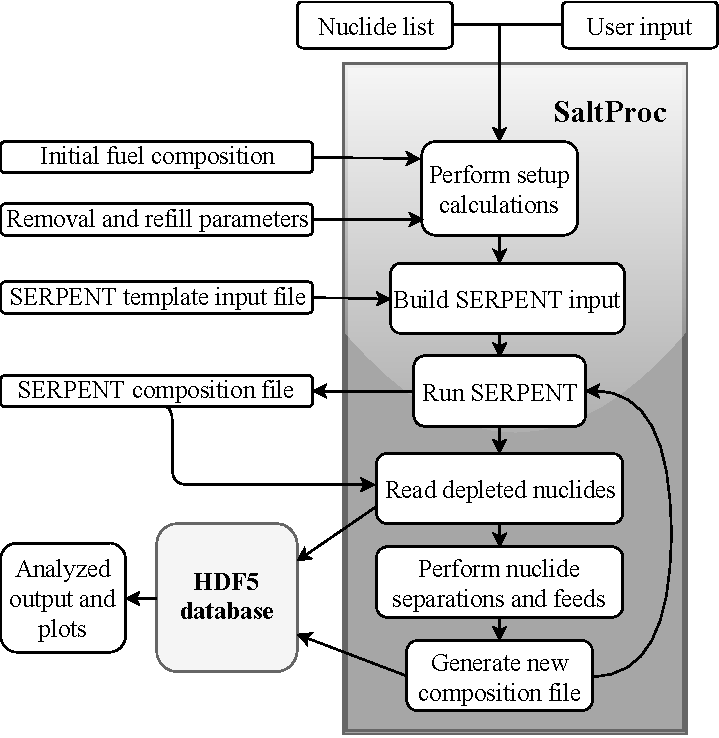
\includegraphics[width=0.75\textwidth]{saltproc_flowchart.pdf}
  \caption{Flow chart for the Saltproc python package.}
  \label{fig:saltproc_flow}
\end{figure}
SaltProc can manage as many material streams as desired. It also may work with 
multiple depletion materials. At the end of each depletion step, SaltProc 
reads the depleted compositions and tracks each material stream individually. 
Following this, it applies chemical separation functions to fuel stream 
vectors. These vectors then form a matrix (isotopics x timesteps) which 
SaltProc stores in an HDF5 database and prints into the SERPENT 2 composition 
file for the next depletion calculation.

SaltProc records every value every timestep. The resulting time series datasets
produced by SaltProc are listed below,
where the values inside the parenthesis are the dataset sizes:

\begin{itemize}
    \item \texttt{core adensity before reproc} (number of isotopes x timesteps)
    \item \texttt{core adensity after reproc} (number of isotopes x timesteps)
    \item \texttt{Keff\_BOC} (1 x timesteps)
    \item \texttt{Keff\_EOC} (1 x timesteps)
    \item \texttt{Th tank adensity} (number of isotopes x timesteps)
    \item \texttt{iso codes} (number of isotopes x 1)
\end{itemize}

In addition, SaltProc is able to define time-dependent material feed and 
removal rates to investigate their impacts. These rates need not be 
constant in SaltProc. They can be defined as piecewise functions or set to 
respond to conditions in the core. For instance, SaltProc might increase the 
fissile material feeding rate if the effective multiplication factor, 
$k_{eff}$, falls below a specific limit (e.g., 1.002).
These capabilities allow SaltProc to analyze fuel cycle of a generic 
liquid-fueled \gls{MSR}. In summary, the development approach of SaltProc 
focused on producing a generic, flexible and expandable tool to give the 
SERPENT 2 Monte Carlo code the ability to conduct advanced in-reactor fuel 
cycle analysis as well as simulate a myriad of online refueling and fuel 
reprocessing systems.
